\documentclass[11pt]{article}
\usepackage[margin=1in]{geometry}
\usepackage{amsmath,amssymb,mathtools}
\usepackage{enumitem}
\usepackage{tikz}
\usetikzlibrary{positioning,calc}

\setlist[itemize]{topsep=2pt,itemsep=2pt}
\setlist[enumerate]{topsep=4pt,itemsep=4pt}
\newcommand{\argmin}{\operatorname*{arg\,min}}
\DeclareMathOperator{\desc}{desc}
\DeclareMathOperator{\chld}{chld}

\title{Assignment 2: Informed Search}
\author{}
\date{}

\begin{document}
\maketitle
\vspace{-3em}

\begin{enumerate}[label=\textbf{\arabic*.}, leftmargin=*]
    \item \textbf{(15 points)} Suppose that we are given an admissible heuristic function $h$. Consider the following function
    \[
        h'(n) =
        \begin{cases}
            h(n), & \text{if } n \text{ is the initial state } s,\\[4pt]
            \max\{h(n),\, h'(n') - c(n',n)\}, & \text{where } n' \text{ is the predecessor node of } n,
        \end{cases}
    \]
    where
    \[
        c(n',n) \coloneqq \min_a c(n',a,n).
    \]
    Prove that $h'$ is consistent.

    \textbf{Solution:}\\
    From the problem, we know that the definition of $h'$, for non-initial node $n$ with predecessor $n'$, 
\[h'(n) = max\{h(n), h'(n') - c(n', n)\}\]
    Since the maximum of this two is at least as large as each of them, we have:
\[h'(n) \ge h'(n') - c(n', n) \]
\[h'(n') \le h'(n) + c(n', n)\]
Since
\[
c(n',n)=\min_a c(n',a,n)\le c(n',a,n)
\]
for every action $a$, we have
\[
h'(n')\le h'(n)+c(n',n)\le h'(n)+c(n',a,n).
\]
Therefore,
\[
h'(n')\le c(n',a,n)+h'(n),
\]
which is exactly the definition of consistent. Therefore, $h'$ is consistent.
    \newpage

    \item \textbf{(25 points)} Consider a search problem over a graph $G = (N,E,C)$, where $N$ are nodes, $E$ are directed edges between nodes, and the weight of an edge $e \in E$ is given by $c(e)$, where $c(e) > 1$, for all $e \in E$. We assume that there is a unique goal state $g$.
    \begin{enumerate}[label=(\alph*)]
        \item \textbf{(5 points)} Consider the heuristic $h_1$ that counts the number of edges between a given state $s$ and the goal state $g$. Show that $h_1$ is consistent.
        \item \textbf{(4 points)} Find a consistent heuristic $h_2$ that dominates the heuristic $h_1$. The heuristic $h_2$ cannot be equal to $h_1$, nor can it be the optimal heuristic $h^*$ that computes the true cost of reaching $g$ from the state $s$.
        \item \textbf{(8 points)} Suppose that we add edges between states in the graph $G$, but keep the heuristic $h_1$ unchanged. Is $h_1$ still admissible and consistent? Prove this claim or give a counterexample.
        \item \textbf{(8 points)} Suppose that we remove edges from the graph $G$, but keep the heuristic $h_1$ unchanged. Is the heuristic still admissible and consistent? Prove this claim or give a counterexample.
    \end{enumerate}
    
    \textbf{Solution:}\\
    \textbf{a)}\\
    Assume $h_1(s)$ is the min number of edges from $s$ to the goal state $g$.\\
    Let's we take a successor of $s$, which is $t$, then we have: $1 + h_1(t)$.\\
    Since $h_1(s)$ is the min number of edges from $s$ to g, we have:
    \[h_1(s) \le 1 + h_1(t)\]
    Because every edge cost $c(e) \ge 1$,
    \[h_1(s) \le 1 + h_1(t) \le c(s, t) + h_1(t)\]
    Hence $h_1$ is consistent.

    \textbf{b)}
\[c_{min} = min_{e \in E} c(e)\]
\[c_{min} > 1\]
Choose a constant $\alpha$
\[1 < \alpha < c_{min}\]
\[h_2(s) = \alpha h_1(s) \text{ and } h_2(s) \ge h_1(s)\]
    Let's we take a successor of $s$, which is $t$, then we have: $1 + h_1(t)$.\\
    Since $h_1(s)$ is the min number of edges from $s$ to g, we have:
    \[h_1(s) \le 1 + h_1(t)\]
    \[h_2(s) \le \alpha + h_2(t)\]
    Since $\alpha \le c(s, t)$,
    \[h_2(s) \le c(s, t) + h_2(t)\]
    Hence $h_2$ is consistent.

    \textbf{c)}
    No\\
    Counterexample:\\

Let we assume a graph:
\[A \rightarrow B \rightarrow g\]
and each edge cost 2.
\[h_1(A) = 2, h_1(B) = 1, h_1(g) = 0\]

Now, we add one more edge $e(A, g)$, and we set the cost $c(A, g) = 1.5$.

Let we check admissible:
\[h^*(A) = 1.5\]
\[h_1(A) = 2 > 1.5 = h^*(A)\]
$h_1$ is not admissible.

Let we check consistent:
\[h_1(A) \le c(A, g) + h_1(g)\]
\[2 \le 1.5 + 0\]
$h_1$ is not consistent.

    \textbf{d)}
Still Admissible and consistent\\

Let we check admissible:\\
Removing edges will not produce a shorter path; it can only make the optimal cost larger or unchanged.
Assume the optimal cost of old graph is $h^*_{odd}(s)$, the optimal cost of new graph is $h^*_{new}(s)$, we have:
\[h^*_{new}(s) \ge h^*_{old}(s)\]
\[h_1(s) \le h^*_{odd}(s) \le h^*_{new}(s)\]
$h_1$ is admissible.

Let we check consistent:\\
New graph edge set: $E_{new}$\\
Old graph edge set: $E_{old}$
\[E_{new} \subseteq E_{old}\]
\[h_1(s) \le c(s, t) + h_1(t) \quad \forall (s, t) \in E_{old}\]
Since every edge in the new graph is also an edge in the old graph, we have:
\[h_1(s) \le c(s, t) + h_1(t) \quad \forall (s, t) \in E_{new}\]
$h_1$ is consistent.
    
    \newpage

    \item \textbf{(20 points)} Answer the following questions.
    \begin{enumerate}[label=(\alph*)]
        \item \textbf{(10 points)} Prove that if $h$ is consistent, then it must be admissible (remember that for any goal state $t$, $h(t) = 0$).
        \item \textbf{(10 points)} Suppose that $h,h'$ are heuristics such that $h$ dominates $h'$. Show that if $h$ is admissible, then so is $h'$; does the same claim hold for consistent heuristics? I.e. if $h$ is consistent and dominates a heuristic $h'$, is $h'$ consistent as well? Prove or provide a counterexample.
    \end{enumerate}
    \textbf{Solution:}\\
\textbf{a)}\\
Let \(n\) be any node, and let
\[
n = n_0 \to n_1 \to \cdots \to n_k = t
\]
be an optimal path from \(n\) to a goal node \(t\). Since \(h\) is consistent, for every edge \((n_i, n_{i+1})\),
\[h(n_i) \le c(n_i, n_{i+1}) + h(n_{i+1})\]
\[h(n_0) \le c(n_0, n_1) + c(n_1, n_2) + \cdots + c(n_{k-1}, n_k) + h(n_k)\]
\[h(n_0) \le c(n_0, n_1) + c(n_1, n_2) + \cdots + c(n_{k-1}, n_k)\]

The right-hand side is the optimal cost from \(n\) to a goal node, which is \(h^*(n)\). Therefore,
\[
h(n) \le h^*(n)
\]
Hence \(h\) is admissible.

\textbf{b)}\\
\textbf{1.}\\
Since \(h\) dominates \(h'\),
\[
h'(n) \le h(n)
\]
Since \(h\) is admissible,
\[
h(n) \le h^*(n)
\]
Therefore,
\[
h'(n) \le h(n) \le h^*(n)
\]
Therefore \(h'\) is admissible.\\

\textbf{2.}\\
No\\
Counterexample:\\
\[
A \to B \to G, 
\qquad c(A,B)=1,\quad c(B,G)=1
\]
Let \(G\) be the goal node.

Define $h$
\[
h(G)=0,\qquad h(B)=1,\qquad h(A)=2
\]
Then \(h\) is consistent:
\[
h(A)=2 \le 1+h(B)=2
\]
\[
h(B)=1 \le 1+h(G)=1
\]
Now define $h'$
\[
h'(G)=0,\qquad h'(B)=0,\qquad h'(A)=2
\]
\[
h'(n)\le h(n)
\]
\(h\) dominates \(h'\).

However,
\[
h'(A)\le c(A,B)+h'(B)
\]
\[
2 \nleq 1+0
\]
Therefore, \(h'\) is not consistent.






    \newpage

    \item \textbf{(20 points)} You have learned before that $A^*$ using graph search is optimal if $h(n)$ is consistent. Does this optimality still hold if $h(n)$ is admissible but inconsistent? Using the graph in Figure~\ref{fig:heuristic-search}, let us now show that $A^*$ using graph search returns a sub-optimal solution path $(S,B,G)$ from start node $S$ to goal node $G$ with an admissible but inconsistent $h(n)$. We assume that $h(G) = 0$.

    Give nonnegative integer values for $h(A)$ and $h(B)$ such that $A^*$ using graph search returns the non-optimal solution path $(S,B,G)$ from $S$ to $G$ with an admissible but inconsistent $h(n)$, and tie-breaking is not needed in $A^*$.

    \begin{figure}[h]
        \centering
        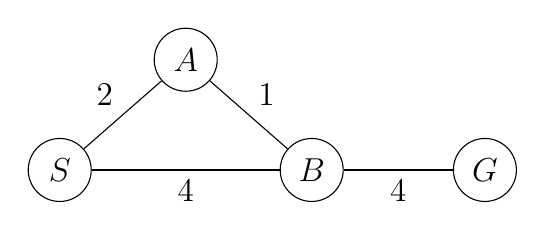
\begin{tikzpicture}[scale=1.0, every node/.style={font=\large}]
            \tikzstyle{state}=[circle, draw, minimum size=8mm, inner sep=0pt]
            \node[state] (S) at (0,0) {$S$};
            \node[state] (A) at (1.6,1.4) {$A$};
            \node[state] (B) at (3.2,0) {$B$};
            \node[state] (G) at (5.4,0) {$G$};
            \draw (S) -- node[above left] {$2$} (A);
            \draw (A) -- node[above right] {$1$} (B);
            \draw (S) -- node[below] {$4$} (B);
            \draw (B) -- node[below] {$4$} (G);
        \end{tikzpicture}
        \caption{Graph for heuristic search.}
        \label{fig:heuristic-search}
    \end{figure}
    \textbf{Solution:}\\
\textbf{a)}\\
Let we take:
\[
h(A)=5,\qquad h(B)=0,\qquad h(G)=0.
\]
\[
h^*(G)=0,\qquad h^*(B)=4,\qquad h^*(A)=1+4=5.
\]
Thus,
\[
h(A)=5\le h^*(A)=5,
\]
\[
h(B)=0\le h^*(B)=4,
\]
\[
h(G)=0\le h^*(G)=0.
\]
Therefore, \(h\) is admissible.
However, \(h\) is not consistent. For edge \(A\to B\),
\[
h(A)\le c(A,B)+h(B)
\]
\[
5\nleq 1+0,
\]
\textbf{b)}\\
\textbf{Step 1:}\\
Expand \(S\),
\[
g(A)=2,\qquad f(A)=g(A)+h(A)=2+5=7,
\]
\[
g(B)=4,\qquad f(B)=g(B)+h(B)=4+0=4.
\]
\[
f(B)<f(A),
\]
A* expands \(B\) first and generates \(G\):
\[
g(G)=4+4=8,\qquad f(G)=8.
\]
\textbf{Step 2:}\\
Expand \(A\), $B$ is already closed.

Then, pop $G$

Therefore, A* returns
\[
(S,B,G)
\]
But the optimal path is
\[
(S,A,B,G)
\]
Thus, $A^*$ using graph search returns a sub-optimal solution path $(S,B,G)$ from start node $S$ to goal node $G$ with an admissible but inconsistent $h(n)$. 

    \newpage

    \item \textbf{(20 points)} Consider the minimax search tree below (Figure~\ref{fig:minimax-tree}). In the figure, black nodes are controlled by the MAX player, and white nodes are controlled by the MIN player. Payments (terminal nodes) are squares; the number within denotes the amount that the MIN player pays to the MAX player (an amount of $0$ means that MIN pays nothing to MAX). Naturally, MAX wants to maximize the amount they receive, and MIN wants to minimize the amount they pay.

    Suppose that we use the $\alpha$-$\beta$ pruning algorithm. Consider the minimax tree given in Figure~\ref{fig:minimax-tree}.
    \begin{enumerate}[label=(\alph*)]
        \item \textbf{(10 points)} Assume that we iterate over nodes from \textbf{right to left}; what are the arcs that are pruned by $\alpha$-$\beta$ pruning, if any?
        \item \textbf{(10 points)} Does your answer change if we iterate over nodes from \textbf{left to right}?
    \end{enumerate}

    \begin{figure}[h]
        \centering
        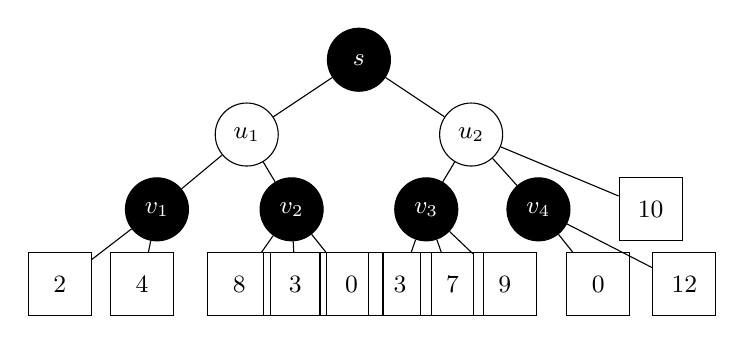
\begin{tikzpicture}[scale=0.95, every node/.style={font=\small}]
            \tikzstyle{maxnode}=[circle, draw, fill=black, text=white, minimum size=8mm, inner sep=0pt]
            \tikzstyle{minnode}=[circle, draw, fill=white, text=black, minimum size=8mm, inner sep=0pt]
            \tikzstyle{leaf}=[rectangle, draw, minimum size=8mm, inner sep=0pt]

            \node[maxnode] (s) at (0,3) {$s$};
            \node[minnode] (u1) at (-1.5,2) {$u_1$};
            \node[minnode] (u2) at (1.5,2) {$u_2$};

            \node[maxnode] (v1) at (-2.7,1) {$v_1$};
            \node[maxnode] (v2) at (-0.9,1) {$v_2$};
            \node[maxnode] (v3) at (0.9,1) {$v_3$};
            \node[maxnode] (v4) at (2.4,1) {$v_4$};
            \node[leaf] (l10) at (3.9,1) {$10$};

            \node[leaf] (l2) at (-4.0,0) {$2$};
            \node[leaf] (l4) at (-2.9,0) {$4$};
            \node[leaf] (l8) at (-1.6,0) {$8$};
            \node[leaf] (l3a) at (-0.85,0) {$3$};
            \node[leaf] (l0a) at (-0.1,0) {$0$};
            \node[leaf] (l3b) at (0.55,0) {$3$};
            \node[leaf] (l7) at (1.25,0) {$7$};
            \node[leaf] (l9) at (1.95,0) {$9$};
            \node[leaf] (l0b) at (3.2,0) {$0$};
            \node[leaf] (l12) at (4.35,0) {$12$};

            \draw (s) -- (u1);
            \draw (s) -- (u2);
            \draw (u1) -- (v1);
            \draw (u1) -- (v2);
            \draw (u2) -- (v3);
            \draw (u2) -- (v4);
            \draw (u2) -- (l10);
            \draw (v1) -- (l2);
            \draw (v1) -- (l4);
            \draw (v2) -- (l8);
            \draw (v2) -- (l3a);
            \draw (v2) -- (l0a);
            \draw (v3) -- (l3b);
            \draw (v3) -- (l7);
            \draw (v3) -- (l9);
            \draw (v4) -- (l0b);
            \draw (v4) -- (l12);
        \end{tikzpicture}
        \caption{A minimax search tree.}
        \label{fig:minimax-tree}
    \end{figure}
\textbf{Solution:}\\
Minmax value: 9

\textbf{a)}\\
Pruned:
\[v_4 \to 0\]
\[u_1 \to v_1\]

\textbf{b)}\\
Pruned:
\[v_2 \to 3\]
\[v_2 \to 0\]









\newpage

    \item \textbf{(Optional, bonus points)} In this question, we will formally prove that the minimax algorithm described in class produces an equilibrium. An extensive form game is defined by a set of nodes $V$ and a set of directed edges $E$, defining a tree. The root of the tree is the node $r$. Let $V_{\max}$ be the set of nodes controlled by the MAX player and $V_{\min}$ be the set of nodes controlled by the MIN player. We often refer to the MAX player as player $1$, and to the MIN player as player $2$. Furthermore, let $\desc(v)$ be the descendants of a node $v$ in the search tree. A strategy for the MAX player is a mapping $s_1 : V_{\max} \to V$; similarly, a strategy for the MIN player is a mapping $s_2 : V_{\min} \to V$. In both cases, $s_i(v) \in \chld(v)$ is the choice of child node that will be taken at node $v$. We let $S_1,S_2$ be the set of strategies for the MAX and MIN player, respectively.

    The leaves of the minimax tree are payoff nodes. There is a payoff $a(v)$ associated with each payoff node $v$, where $a(v)$ is the amount that the MAX player receives and $-a(v)$ is the amount that the MIN player receives if the node $v$ is reached. The MAX player wants to maximize their payoff, and the MIN player wants to minimize the amount that they pay. More formally, the utility of the MAX player from $v$ is $u_{\max}(v) = a(v)$ and the utility of the MIN player is $u_{\min}(v) = -a(v)$. The utility of a player from a pair of strategies $s_1 \in S_1, s_2 \in S_2$ is simply the utility they receive by the leaf node reached when the strategy pair $(s_1,s_2)$ is played.

    \paragraph{Definition 1 (Nash Equilibrium).} A pair of strategies $s_1^* \in S_1, s_2^* \in S_2$ for the MAX player and the MIN player, respectively, is a Nash equilibrium if no player can get a strictly higher utility by switching their strategy. In other words:
    \[
        \forall s \in S_1 : u_1(s_1^*,s_2^*) \ge u_1(s,s_2^*);
    \]
    \[
        \forall s' \in S_2 : u_2(s_1^*,s_2^*) \ge u_2(s_1^*,s').
    \]

    \paragraph{Definition 2 (Subgame).} Given an extensive form game $\langle V,E,r,V_{\max},V_{\min},\vec{a}\rangle$, a subgame is a subtree of the original game, defined by some arbitrary node $v$ set to be the root node, and all of its descendants (i.e. its children, its children's children etc.), denoted by $\desc(v)$. Leaf nodes and node control are the same as in the original extensive form game.

    \paragraph{Definition 3 (Subgame-Perfect Nash Equilibrium (SPNE)).} A pair of strategies $s_1^* \in S_1, s_2^* \in S_2$ is a sub-perfect Nash equilibrium if it is a Nash equilibrium for any subtree of the original game tree.

    \begin{enumerate}[label=(\alph*)]
        \item Prove that the minimax algorithm shown in class outputs a subgame-perfect Nash equilibrium.
        \item Consider a node $v$ in an adversarial search problem. Assume that $v$ is controlled by the MAX player (Player 1). Prove that $\alpha$-$\beta$ pruning only removes subtrees of $v$ that offer Player 1 a payoff that is weakly lower than their payoff in the subtree rooted in $v$ under a subgame-perfect Nash equilibrium.
    \end{enumerate}
\end{enumerate}

\end{document}
